\documentclass[border=2pt]{standalone}
\usepackage{pgfplots}
\begin{document}
	
    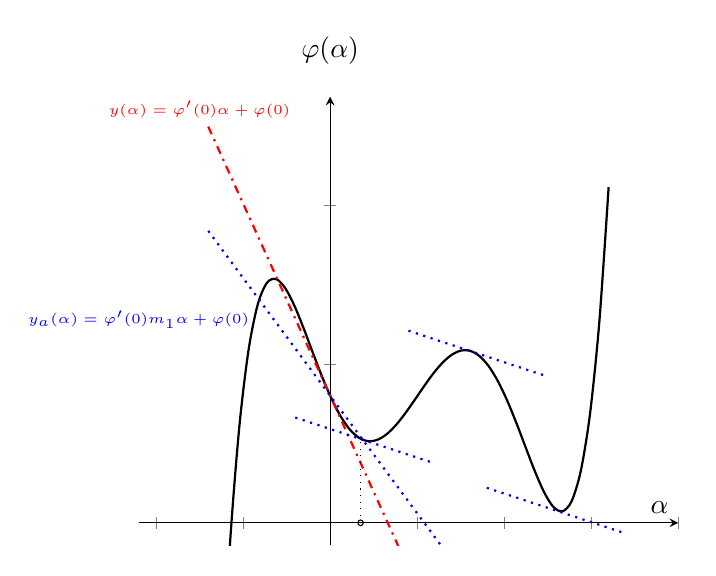
\begin{tikzpicture}[declare function={
    	f(\x)=0.988*\x^5-4.96*\x^4+4.978*x^3+5.015*x^2-6.043*x+4;
    	a(\x) = -3.7*\x + 4;
    	df(\x)=-6.043*\x +4;
    	t1(\x) = -.9*\x + 2.95;
    	rt1(\x) = 0.9*\x + 2.1;
		t2(\x) = -.9*\x + 6.85;
		rt2(\x) = 0.9*\x + 4.08;
		t3(\x) = -.9*\x + 2.72;
		rt3(\x) = 0.9*\x + -2.04;
    	g(\x) = -2.9*\x + 4;
    	i(\x) = 0;}]
        \begin{axis}[
            % center the x axis
            axis x line=middle,
            % we don't need a y axis line ...
            axis y line=middle,
            % ... and thus there is no need for much `height' of the axis
            %height=150pt,
            % but `height' also changes `width' which is restored here
            %width=\axisdefaultwidth,
            xmin=-2.2,
            xmax=4,
            ymin=-0.7,
            ymax=13.4,
            ylabel style={rotate=-90},
            xticklabels={,,},
            yticklabels={,,},
            xlabel={$\alpha$},
            ylabel={$\varphi(\alpha)$},
            samples=50,
            every axis y label/.style={
            	at={(ticklabel* cs:1.05)},
            	anchor=south,
            }
        ]
        
	  \addplot[domain=-2:3.2,thick,smooth] (x,{f(x)});
	  
	  \addplot[domain=-1.4:4.2,thick,dashdotted,red] (x,{df(x)});
	  \addplot[mark=text, mark options={fill=red}, text mark={\tiny $y(\alpha) = \varphi'(0)\alpha + \varphi(0)$}] coordinates {(-1.5, 13)};
	  
	  \addplot[domain=-1.4:4.2,thick,dotted, blue] (x,{a(x)});
	  \addplot[mark=text, mark options={fill=blue}, text mark={\tiny $y_{\tiny a}(\alpha) = \varphi'(0) m_1\alpha + \varphi(0)$}] coordinates {(-2.2, 6.4)};
	  
	    
	  \addplot[domain=-.4:1.2,thick,dotted, blue] (x,{t1(x)});
	  \addplot[domain=.9:2.5,thick,dotted, blue] (x,{t2(x)});
	  \addplot[domain=1.8:3.4,thick,dotted, blue] (x,{t3(x)});
	  
	  
	  \addplot[mark=o,mark size=1,mark options={fill=black}] coordinates {(0.35, 0)} node{};
	  \addplot[mark=none,mark size=.8,mark options={fill=black},dotted] coordinates {(0.35, 0) (0.35, 2.58)} node{};
	
        \end{axis}
    \end{tikzpicture}
\end{document}